% Appendix B. Source: Appendix 4.A of Dissertation/Chapter4_Methodology.md.

\chapter{The Tracker, its Structure and its Cleaning}
\label{app:tracker}
\lhead{Appendix B. \emph{The Tracker and its Cleaning}}

Source, unmodified: \texttt{CTIMP Trials 150 Day Metric Tracker- 2026-07-30 SE.xlsx}. Outputs: a cleaned table holding one row per trial, a model-ready extract of the fields the model uses, and the log this appendix summarises. The source file was not edited at any point, so every output is a derivative and a corrected tracker can be processed by re-running the script.

\textbf{What the tracker is.} The CTIMP 150-day metric tracker is maintained in Research and Innovation and reported against the national targets. Its Report sheet holds one row per trial across 23 columns, of which the pharmacy block runs from the day the Research Setup and Governance meeting notifies pharmacy to the day pharmacy issues its greenlight. A second sheet, Raw data, holds 2,666 rows covering the whole portfolio including declined and closed studies, and is used only to estimate the arrival rate, since studies that never reached set-up carry no pharmacy milestones.

\textbf{How the pharmacy dates get into it.} By hand, from emails, local folders and the trust's quality system, with the aseptic figures arriving separately from the Pharmacy Quality Lead. None of it is a system export, so a blank records a retrieval failure rather than an event that did not happen. Two consequences. The aseptic sign-off is a tick on a whiteboard, so there is no date to retrieve. And trials before 2023 carry only HRA approval, site selected and the open-to-recruitment date, the pharmacy fields not being collected then; since those two are the clock anchors, an old trial's deadline is computable while its duration is not.

\textbf{What the tracker does not hold.} Across the 104 distinct trials the cleaned file holds 28 pharmacy notification dates and 24 pharmacy green lights, no PPCTI sign-off dates at all, and 9 trials with no complexity tier. Figure~\ref{fig:completeness} sets every field against the rest. The gap is structural rather than random, but it does not fall where the obvious reading suggests. It tracks whether a record is held in a system, not which team owns the field. iQemo is pharmacy's own and is a digital system, and its dates are present for 51 of the 104 trials, better populated than 5 of the 9 fields arriving from outside pharmacy. The aseptic PPCTI sign-off, kept as a tick on a whiteboard, is empty for all 104. What cannot be retrieved is what was never written into a system, which is why chasing pharmacy would not have produced these dates and why the case studies were requested instead.

\begin{figure}[htbp]
  \centering
  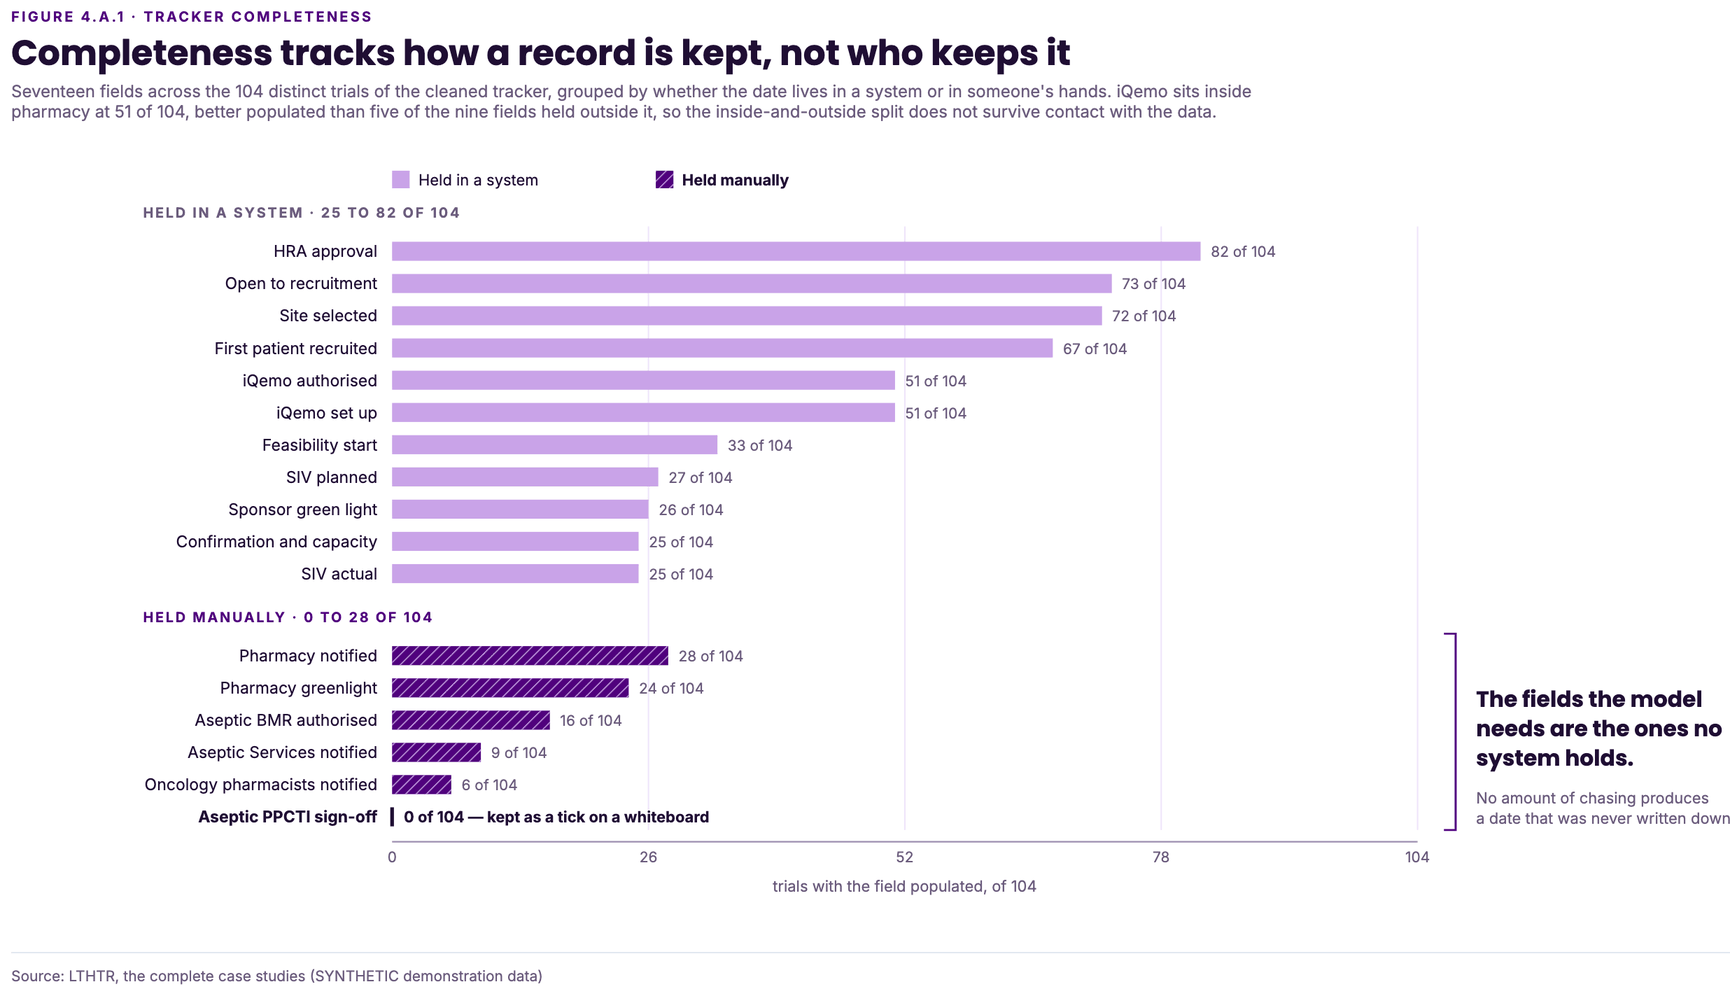
\includegraphics[width=\textwidth]{fig4_A1_tracker_completeness.png}
  \caption[Field completeness across the cleaned tracker]{Field completeness
  across the cleaned tracker, grouped by how each record is kept. Seventeen
  fields are shown against the 104 distinct trials of the cleaned file, split
  into a system-held group ranging from 25 to 82 and a manually held group
  ranging from 0 to 28. The aseptic PPCTI sign-off has no bar at all. A blank
  is a date that could not be retrieved, not a step that did not happen.}
  \label{fig:completeness}
\end{figure}

\textbf{One field reported and then set aside.} Confirmation and capacity to the \emph{sponsor's} green light has a median of exactly one day across the 23 trials holding both dates. That is not a measure of governance speed. The trust's own account is that the sponsor's green light is an announcement made once everything else is complete, so the one day measures the announcement, not the process behind it. It is a different event from the pharmacy green light of Section~\ref{sec:casestudies}, which ends set-up; the two are months apart and only the second bounds segment C. It is recorded here so that no reader treats it as evidence that governance is fast.

\begin{table}[htbp]
  \centering
  \caption{The four faults and their treatment}
  \label{tab:faults}
  \begin{tabularx}{\textwidth}{@{}LlL@{}}
    \toprule
    \textbf{Fault} & \textbf{Extent} & \textbf{Treatment} \\
    \midrule
    Trials stored as two half-filled rows & 14 pairs &
      Merged on a normalised title, each field taking the single non-empty
      value available \\
    \addlinespace
    ``As above'' in place of a date & 18 cells &
      Replaced with the value in the row above, which is what the phrase
      refers to \\
    \addlinespace
    Dates held as \texttt{dd/mm/yyyy} text & 19 cells & Parsed to real dates \\
    \addlinespace
    ``Pending'' in a date column & 4 cells &
      Left blank, since it is not a date \\
    \bottomrule
  \end{tabularx}
\end{table}

The two positional and text faults were the more damaging of the four relative to their size. All 18 ``as above'' cells and 8 of the 19 text dates sat in the pharmacy columns, so nearly the whole of both notification columns was invisible to any calculation that read them as dates.

\textbf{How the split rows were merged.} Rows were grouped on the trial title reduced to lower case with punctuation and bracketed protocol codes removed. Within a group each field took the single non-empty value available, and the longer title was kept because it carries the protocol code. Eleven of the 14 pairs merged with no conflict at all. Most apparent conflicts elsewhere were an ``as above'' against a real date, or a text date against the same date stored properly, and both dissolve once the other 2 faults are corrected.

\textbf{The three unresolved trials.} Where the two rows of a pair disagreed on a real value, the field was left blank and logged. AMPLITUDE differs by 2 to 3 years on 4 fields, with both sets internally consistent, which suggests two different studies sharing a short title rather than one split record. TAK-079-3001 differs on 3 fields, one of which looks like a transposed day and month while the others do not. Orion-BC differs by one day on a feasibility start date and affects no model quantity. Only the second costs anything: its blanked pharmacy green light removes the trial from the sample of measurable pharmacy durations.

\begin{table}[htbp]
  \centering
  \caption{What the clean-up changed}
  \label{tab:cleanup}
  \begin{tabular}{@{}lll@{}}
    \toprule
    \textbf{Quantity} & \textbf{Before} & \textbf{After} \\
    \midrule
    Distinct trials & 118 & 104 \\
    Pharmacy set-up sample & 24 & 23 \\
    Set-up median & 96 days & 95 days \\
    Set-up mean & 105.7 days & 105.9 days \\
    Within 60 days & 2 of 24 & 2 of 23 \\
    Work in progress, mean & 3.41 & 3.51 \\
    Arrival rate & 0.97 per month & 1.00 per month \\
    Trials carrying a complexity tier & 90.7 per cent & 91.3 per cent \\
    \bottomrule
  \end{tabular}
\end{table}

\textbf{An internal consistency check.} An arrival rate of 1.00 trials per month against a 95-day median sojourn implies 3.48 trials in progress by Little's Law, against 3.51 observed, a gap of 0.9 per cent. It is the only check available on the cleaned tracker that does not depend on the fields the trust cannot supply.

\textbf{What was left alone, and why.} 4 items were not repaired because repair would mean invention rather than correction: the PPCTI column, empty for all 104 trials because the step is recorded as a tick on a whiteboard; 9 trials with no complexity tier, which cannot be inferred; the sparse pharmacy dates, since cleaning cannot create a record that was never made; and the three conflicts above. The start of the 60-day clock is also untouched, being a definition rather than a data fault.
